% Created 2018-10-09 Tue 14:49
% Intended LaTeX compiler: pdflatex
\documentclass[11pt]{article}
\usepackage[utf8]{inputenc}
\usepackage[T1]{fontenc}
\usepackage{graphicx}
\usepackage{grffile}
\usepackage{longtable}
\usepackage{wrapfig}
\usepackage{rotating}
\usepackage[normalem]{ulem}
\usepackage{amsmath}
\usepackage{textcomp}
\usepackage{amssymb}
\usepackage{capt-of}
\usepackage{hyperref}
\author{Jacob Sonnenberg}
\date{\today}
\title{SOD Assignment 1: Revisited}
\hypersetup{
 pdfauthor={Jacob Sonnenberg},
 pdftitle={SOD Assignment 1: Revisited},
 pdfkeywords={},
 pdfsubject={},
 pdfcreator={Emacs 27.0.50 (Org mode 9.1.14)}, 
 pdflang={English}}
\begin{document}

\maketitle
\tableofcontents

\section{Introduction}
\label{sec:org8e1c2ff}
\subsection{Purpose}
\label{sec:org554539a}
This document presents a design aimed at reducing waste, caused by
a university cafeteria over-producing food, by using a pre-ordering
service along with historical analysis to provide accurate
short-term demand estimates as well as insight into overall trends.
\subsection{Assumptions}
\label{sec:orgdb4b367}
\subsection{Terminology}
\label{sec:org9f843d0}
\section{Business Domain}
\label{sec:org4272c87}
\subsection{Model}
\label{sec:org4db7db3}
\begin{center}
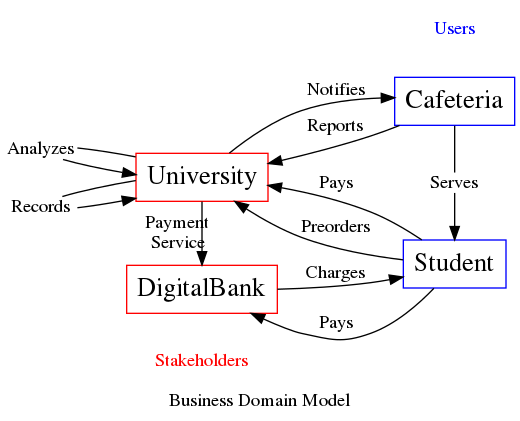
\includegraphics[width=.9\linewidth]{res/business_domain.png}
\end{center}

\subsection{Participants}
\label{sec:org8590530}

\subsubsection{Stakeholders}
\label{sec:orga18f928}
\begin{enumerate}
\item \textbf{University ::}
\label{sec:org0212f64}
The university will provide a preordering service for students
and a notification service for the Cafeteria, informing it of
students' orders.

Additionally the University will be recording transactions made
through the preorder service (and those made without it) so that
the data may later be analyzed.
\item \textbf{Digital Payment Processor ::}
\label{sec:org6ad8f9f}
A Digital Payment Processing company provides exactly such a
service, processing pre-order payments made through an online
service.
\end{enumerate}
\subsubsection{Users}
\label{sec:orgaa2e37c}
\begin{enumerate}
\item \textbf{Cafeteria ::}
\label{sec:org9500b49}
The Cafeteria serves food to Students, receiving orders directly
from a student or indirectly via the University's preorder
service. The Cafeteria produces the supply.
\item \textbf{Students ::}
\label{sec:org531929c}
A Student of the University is a customer of the
Cafeteria. Students generate demand.
\end{enumerate}
\subsection{Potential Services}
\label{sec:org008c3fb}
\subsubsection{Preorder Service}
\label{sec:org35d391e}
The service by which Students can communicate their demand ahead
of time.
\begin{enumerate}
\item \textbf{Authorization Service ::}
\label{sec:org5aa266d}
Provided by the University for the Students, Cafeteria, and
University Administrators. Serves as a security gateway for
accessing software components of the system.
\item \textbf{Online Ordering Service ::}
\label{sec:org339dedf}
Provided by the University for the Students. An internet gateway
Students use to interact with the system.
\item \textbf{Notification Service ::}
\label{sec:org4dbb3cc}
Provided by the University to the Cafeteria. Informs the
Cafeteria of what orders have been placed, the contents of the
order and the desired pickup time.
\item \textbf{Digital Payment Service ::}
\label{sec:org429fd58}
Provided by the Digital Bank stakeholder, if the Student pays at
the time of preordering, they are transferred to the Digital
Bank's service in order to complete the payment.
\item \textbf{Service Service ::}
\label{sec:orgf215de6}
Non-software service provided the Cafeteria, performing food
preparation and acting as the point of sale.
\end{enumerate}
\subsubsection{Prediction Service}
\label{sec:org4d46ec9}
The service by which a prediction of demand in the short and long
term is made.
\begin{enumerate}
\item \textbf{Analysis Service ::}
\label{sec:org4d76ca1}
Owned by the University
\item \textbf{Record Service ::}
\label{sec:orgb215e4c}
Owned by the University. Records orders made through the preorder
service as well as local sales made by the cafeteria, either
automatically or manually updated.
\end{enumerate}
\subsection{Usage Scenarios}
\label{sec:org06b632e}
\subsubsection{Use Case 1}
\label{sec:org3bec0e6}
\subsubsection{Use Case 2}
\label{sec:org0362ea8}
\section{Functional Requirements}
\label{sec:org4cd644b}
\section{Quality Requirements}
\label{sec:orgd749fb0}
\section{Business Services}
\label{sec:org75e9ecb}
\section{Design Space}
\label{sec:org4741617}
\section{Sustainability Strategies}
\label{sec:org8094603}
\end{document}
